\chapter{Introduccion a Big Data}
\rule{\textwidth}{3pt}\\[10ex]

En el capitulo 2 vamos a centrarnos en explicar y  analizar el concepto Big Data. ¿Qué es Big Data? ¿Cuándo y por qué ha surgido este nuevo término en el campo de las TIC? ¿Para qué sirve? ¿Es importante? y la incógnita principal de todo nuevo campo tecnológica ¿Podemos sacar beneficios con el Big Data?
\\[1cm]
\section{Concepto y evolución histórica}

Según el  primer estándar internacional de la ITU(International Telecommunication Union) para Big Data aprobado en Diciembre del año 2015 por el grupo de expertos responsables de las redes futuras, el cloud computing y los aspectos relacionados con las redes de comunicaciones móviles, ITU-T Study Group 13, la definición oficial de Big data es:\\

\emph{Big Data is a paradigm for enabling the collection, storage, management, analysis and visualization, potentially under real-time constraints, of extensive datasets with heterogeneous characteristics.}\\
\\
\textit{Big Data es un paradigma para hacer posible la recopilación, el almacenamiento, la gestión, el análisis y la visualización, potencialmente en condiciones de tiempo real, de grandes conjuntos de datos con características heterogéneas.}
\cite{ITU_standard}\\

Abstrayéndonos de la definición general, el Big Data tiene se origen de algo tan simple y antiguo como es el almacenamiento y uso de grandes cantidades de datos.
Desde las primeras bibliotecas en la antigua Roma o los mecanismos primitivos usados para controlar la actividad comercial, ya se hacía uso del almacenamiento de datos para poder usarlos  posteriormente, aunque la cantidad de datos fuera mucho menor que cuando hablamos de Big Data.Este es una de las características principales cuando hablamos de Big Data, la enorme cantidad de datos que vamos a tratar.\\

Será a finales de la década de 1990 y a principios del nuevo milenio cuando se empiece a hablar  del termino Big Data tal y como lo entendemos hoy en día. Fue el informático estadounidense \emph{John Mashey} él que empezó a hablar del termino Big Data en un artículo publicado con título \emph{Big Data and Next Wava of Infrastress} donde ya predecía la avalancha de datos que se vendría en los años siguientes, la importancia de los mismos y la necesidad de desarrollar nuevas tecnologías para poder hacer frente a la inmensa cantidad de datos. Durante los próximos años se experimentaría un incremente bastante  significativo en el número de datos online ocasionados por la nueva era de internet con la web 2.0, además ya se empezará a hablar del denominado internet de las cosas.
\cite{John_Mashey}\\

Desde entonces, y hasta ahora, el uso del Big Data solo ha aumentado, provocado en gran medida por el gran aumento en el número  de datos que generamos.\\
Para hacernos una idea, según la Unión Europea, hoy día se generan 17000 billones de bytes por minutos, unos seis megabytes por persona y día. Además, según un estudio realizado por IDC y patrocinado por EMC, de 2005 a 2020 se espera que el tamaño del universo digital se multiplique por 300, creciendo de 130 exabytes a 40 mil.
\cite{IDC}\\

\begin{figure}[H]
	\centering
	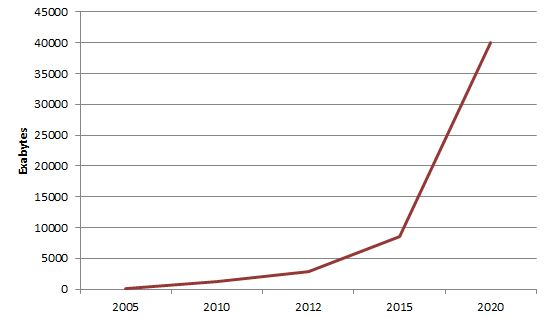
\includegraphics[width=0.7\textwidth]{./imagenes/evolucion_datos}
	\caption{Cantidad de datos digitales (exabytes) desde 2005 a 2020\cite{IDC}} 
	
\end{figure}


Cada vez son más los campos empresariales en los que se hace casi imprescindible saber almacenar los datos y saber cómo analizarlos de forma correcta. Expertos en áreas como la bolsa, investigación o el marketing cada vez son más conscientes de que el futuro está saber analizar de forma correcta la enorme cantidad de datos que recopilan. En secciones posteriores de este mismo capítulo trataremos la importancia del mercado del Big Data en la actualidad.

\section{Características del Big Data}

Podemos hablar de cuatro características principales para definir la información relativa a Big Data, las cuatro Vs del Big Data:\\\\

•	\textbf{Volumen}: Los datos utilizados en Big Data son producidos en enormes cantidades lo que dificulta su análisis. Actualmente, los datos no son solo generados por personas, sino también por todo tipo de maquinaria y sensores, lo que acelera la producción de los mismos. Según un estudio recogido por Qmee, cada 60 segundos se mandan unos 278.000 tuits o se realizan 2 millones de búsquedas en google.
\cite{blog_qmee}
\\

•	\textbf{Velocidad}: La velocidad es referida a la velocidad con lo que se generan nuevos datos para ser analizados y la capacidad de analizar los mismo en el menor tiempo posible. Como hemos visto en el ejemplo anterior, la velocidad con la que se generan nuevos datos es del orden de milisegundos o nanosegundos. Cuanto mayor sea la velocidad a la hora de analizarlos, mayor partido y beneficio podremos hacer de los mimos.
\\

•	\textbf{Variedad}: La variedad de datos que nos podemos encontrar a la hora de hacer un análisis en Big Data es muy extensa, lo que dificulta poder sacar una conclusión clara del mismo. Los datos producidos por personas, sensores o maquinas son de distinta naturaleza, lo que genera la necesidad de crear  nuevos tipos de datos para  facilitar su análisis.
\\

•	\textbf{Veracidad}: Es la características más importante en lo relativo a Big Data. Necesitamos saber si los datos que hemos obtenidos, así como el análisis que hagamos de los mismo, va a ser válido y veraz. Necesitamos diferenciar entre los distintos datos, ya que no todos serán válidos, y entre estos habrá algunos con más valor que otros. \\


\begin{figure}[H]
	\centering
	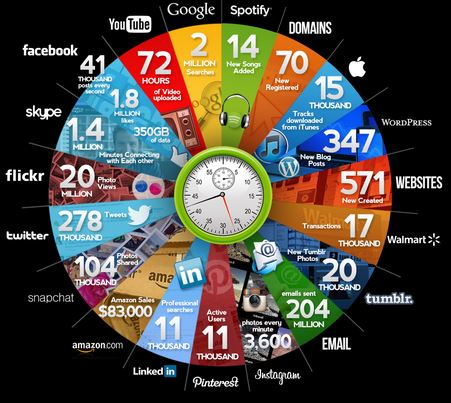
\includegraphics[width=0.5\textwidth]{./imagenes/Estudio_Qmee}
	\caption{Cantidad de datos online en 60 seg. \cite{blog_qmee}} 
	
\end{figure}



\section{Fuentes y tipos de datos}

Como hemos comentado en las secciones anteriores, el uso de Big Data se basa en hacer un análisis a los datos con el fin de sacar conclusiones y resultados que nos ayuden con un fin concreto.\\

Un aspecto a tener muy en cuenta durante el análisis es preguntarnos qué tipo de datos estamos analizando, su procedencia, así como el valor que tendrá cada uno de ellos. Si estamos haciendo un estudio para predecir los posibles resultados de unas elecciones, no podremos tratar de igual forma los datos recogidos por una encuesta a pie de urna y los datos recogidos referentes a el gasto en la campaña de cada partido. Como vemos, tenemos que tener en cuenta la naturaleza de los datos y el valor que les damos a la hora de analizarlos. También tendremos que tener en cuenta qué datos son necesarios para nuestro análisis y cuáles no, ya que por ejemplo a veces necesitaremos datos en tiempo real,  en los sondeos a pie de urna  por ejemplo, y otras veces no necesitaremos los datos de tiempo real, como puede ser el análisis de los datos de ventas de una empresa en las diferentes campañas de moda.\\

Los datos relativos a Big Data se dividen en tres tipos principales, estructurados, semiestructurados y no estructurados.\\

•	\textbf{Datos estructurados}: Son los datos se pueden definir en longitud y formato, como pueden ser fechas, números o datos característicos. Son los datos que normalmente se usan para analizar y sacar conclusiones. La mayoría de expertos cree que los datos estructurados forman el 20\% de los datos producidos.\\

Los datos estructurados los podemos dividir en dos categorías:\\

-	\emph{Generados por máquinas}: Son los datos generados por las máquinas sin ningún tipo de intervención humana. Son datos como los recogidos por sensores y los producidos por servidores o páginas webs.\\

-	\emph{Generados por humanos}: Son los datos generados por los humanos en interacción con las máquinas. Como por ejemplo los datos que generamos cuando entramos a una página web o los que introducimos a una base de datos de un servidor.\\

•	\textbf{Datos semiestructurados}: Los datos semiestructurados son datos que no tienen formato fijo(como los no estructurados), pero contienen etiquetas y marcadores que permiten separar los diferentes datos(como los estructurados). Un ejemplo de datos semiestrucutrados pueden ser los textos de etiquetas de XML o HTML.\\



•	\textbf{Datos no estructurados}: Son los datos que no tienen un formato específico. Suponen un mayor reto para ser analizados, ya que normalmente son analizados de forma manual. La mayoría de los datos que se producen son no estructurados, alrededor del 80\%.\\

Al igual que los datos estructurados, pueden ser divididos en dos categorías:\\

-	\emph{Datos generados por máquinas}: Son los datos que se generan sin intervención humana, como pueden ser datos recogidos por una cámara de seguridad o os de un satélite.\\


-	\emph{Datos generados por humanos}: Algunos ejemplos son los datos que generamos por las redes sociales o los que generamos al enviar mensajes de texto.


\section{Aplicaciones y actualidad del Big Data}

La tecnología Big Data llego para quedarse. Actualmente  son pocas las grandes empresas que no tiene entre sus principales objetivos el desarrollo de un grupo de analistas de Big Data, además, la industria del Big Data no para de crecer.\\

Según Statista,  el valor de mercado del Big Data en 2015 fue de 11.957 millones de euros, y se estima que en 2016 sea de 15.732 millones. \cite{mercado_bigdata} \\

Un dato que refleja a la perfección el aumento de la importancia y la popularidad del Big Data es el interés que tienen los usuarios en él. En la siguiente gráfica se refleja el interés de los usuarios analizando las búsquedas en Google de los temas relacionados con Big Data y Hadoop desde 2004 hasta 2016. Hadoop es la principal herramienta usada para resolver problemas de Big Data, será tratado mas adelante en éste capítulo.\\

\begin{figure}[H]
	\centering
	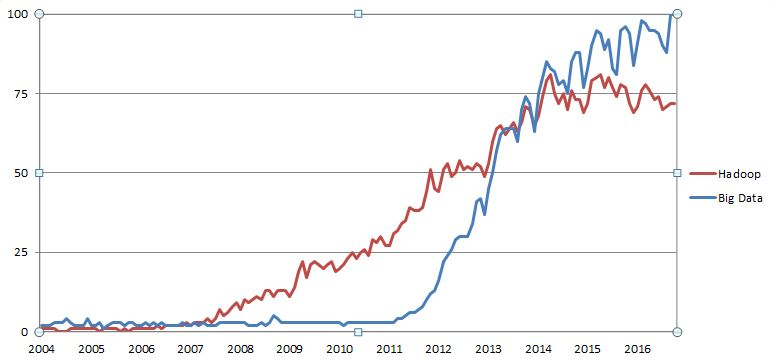
\includegraphics[width=0.8\textwidth]{./imagenes/Interes_Google}
	\caption{Interés sobre Big Data y Hadoop por las búsquedas en Google \cite{Google_trends}} 
	
\end{figure}

Como vemos en la gráfica, el interés por el Big Data, así como por Hadoop, no ha parado de subir con los años, hasta colocarse próxima a 100, lo que significa interés máximo por parte de los usuarios de Google.
También podemos identificar en la gráfica, que fue por los años 2011 y 2012 cuando el interés por el Big Data tiene un aumento significativo por parte de los usuarios, que se corresponde con los años en los que se empieza a hacer popular el termino de Big Data y el denominado internet de las cosas.\\


Pero, por qué el Big Data puede llegar a ser tan importante para una empresa.\\

\emph{Bill Schmarzo} en su libro \emph{Big Data, El poder de los datos}, nos cuenta como a finales de la década de 1980, la empresa Informatio Resources Inc.(IRI) presentó su producto Infoscan, que combinaba los sistemas de escáners de TPV con los códigos de barras, lo que revoluciono el proceso de cadena de valor producto-minorista. El volumen de datos en relación a las ventas de minoristas aumento de megabytes a terabytes.
Hubo empresas como Tesco que aprovecharon esta nueva fuente de datos y las innovaciones relacionadas con la gestión y el análisis de datos para crear aplicaciones como la predicción basada en la demanda, la efectividad de la promoción del comercio, el análisis de la cesta de la compra, la gestión de las rebajas o hasta incluso programas de fidelización de los clientes.\\

Como vemos, gracias al desarrollo de estas nuevas aplicaciones se optimizo mucho más la relación con el minorista, así como la eficiencia de las ventas de sus productos, y además, el análisis de todos estos datos no precisaba grandes periodos de tiempo.\\

Actualmente, una de las aplicaciones de Big Data que más llaman la atención son las relacionadas con el sector del marketing y la publicidad. \\

Queremos comprarnos una bicicleta nueva, y para ello navegamos por internet  en busca de una  bicicleta con las características y el precio que buscamos. A partir de ese momento, y hasta que busquemos otro artículo por internet, toda la publicidad que nos aparecerá en la red estará relacionada con el sector del velocípedo.
Detrás de este ímpetu de internet porque nos compremos una bicicleta nueva, hay un estudio y un análisis de nuestras visitas en internet, los portales que visitamos, las tiendas online a las que hemos acudido en busca de nuestro producto y hasta de la talla o el color que preferimos para nuestra bicicleta.\\

La vicepresidenta de Analíticas y Gestión de la Información de IDC, \emph{Dan Vesset}, explica que \emph{"las empresas que sean capaces de aprovecharse de la nueva generación de soluciones de analítica de negocios, podrán aprovecharse de la transformación digital y adaptarse a los cambios disruptivos, creando una diferenciación competitiva en sus mercados"}, a su vez, \emph{Jessica Goepfert},Directora del Programa de Compresión de Clientes y Analíticas de IDC afirma que \emph{"no existen dudas de que el Big Data y el campo de la analítica supondrán un impacto considerable en casi todas las industrias"}.\\\cite{ingresos_IDC}

En un reciente estudio realizado por IDC aseguran que los ingresos generados por el mercado del Big Data pasarán de 122.000 millones de dolares en 2015 a más de 187.000 millones en 2019, suponiendo un incremento de casi el 50\%, siendo los servicios la parte que más ingresos aportará, seguido de el software y el hardware. \cite{ingresos_IDC}\\

\section{Herramientas}

En esta sección vamos a tratar de introducir las principales herramientas usadas para resolver el problema del Big Data. Nos centraremos principalmente en dos, Hadoop, que es la más conocida y extendida, y Spark, que es la más reciente.\\

•	\textbf{Hadoop}: Apache Hadoop es un framework opensource que permite el procesado de grandes volúmenes de datos de forma distribuida, utilizando para ello una serie de clusters.\\

Hadoop separa y distribuye los datos dividiendo el análisis en tareas más pequeñas que puedan ser abordadas por un ordenador convencional, además, con esta distribución provee de  redundancia y tolerancia a fallos. Todo el proceso de distribución y procesado de los datos es totalmente transparente al usuario. Hadoop hace uso de su \emph{Hadoop Distributed File System}(HDFS) para almacenar los datos, y del algoritmo MapReduce para procesarlos.\\ 

-	\emph{HDFS}: Es un sistema de almacenamiento distribuido pensado para el almacenamiento de grandes volúmenes de datos. Las principales ventajas de HDFS es que provee de redundancia a los datos almacenados y además es tolerante a fallos. Podemos destacar dos tipos de nodos:\\

	\emph{NameNode}: Es único en cada clúster. Se encarga de proveer los datos a los clientes. Contiene las relaciones entre los bloques de datos y los DataNodes en los que están almacenados.\\
	
	\emph{DataNode}: Son los encargados de almacenar los bloques de datos, así como de leer y escribir las peticiones de los clientes.\\
	
	HDFS separa los datos de entrada en diferentes bloques, de 64 MB normalmente, estos bloques de datos son almacenados en tres DataNodes independientes, proveyendo de este modo redundancia de información, y además en el caso de que se caiga un DataNode, la información que tenía almacenada seguirá siendo accesible en otro DataNode. El NameNode tendrá almacenado qué bloques de información tiene almacenado cada DataNode, siendo el encargado de responder a las peticiones del cliente.\\
	
-	\emph{MapReduce}: Es un paradigma de programación desarrollado para la computación distribuida, haciendo uso de la paralelización del procesamiento de grandes volúmenes de datos. Está basado en dos tareas principales, Map y Reduce.\\

La función Map transforma un conjunto de datos de entrada en un numero de pares clave/valor. La salida de la función Map es la entrada de la función Reduce, de forma que esta reduce el número de pares clave/valor combinando las distintas salidas de la función Map que tengan la misma clave.\\

\begin{figure}[H]
	\centering
	\includegraphics[width=0.7\textwidth]{./imagenes/MapReduce}
	\caption{Algoritmo MapReduce} 
	
\end{figure}

Suponemos que el dato de entrada es una frase, por ejemplo “Explicando MapReduce” y queremos saber cuántas veces aparece cada letra.\\

Se dividen los datos de entrada en dos bloques de datos, cada palabra será un bloque en este caso, y lo introducimos en la función map(). El resultado de la función map() nos dará los pares clave/valor que será letra/número de veces que aparece. Los pares clave valor que devuelve la función map() serán la entrada a la función reduce() que combinara los pares con la misma clave.\\

\begin{figure}[H]
	\centering
	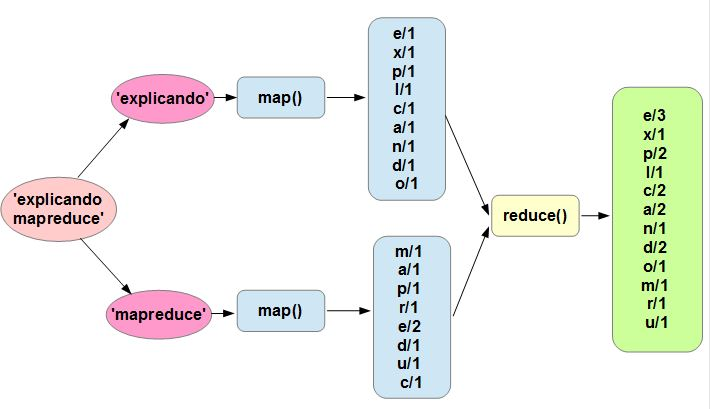
\includegraphics[width=0.7\textwidth]{./imagenes/ejemplo_mapr}
	\caption{Ejemplo MapReduce} 
	
\end{figure}


•	\textbf{Spark}: Apache Spark es un motor de procesamiento de grandes cantidades de datos.\\
 Spark posee una evolución del algoritmo MapReduce de  Hadoop, el cual es mucho más rápido en el procesamiento de los datos.
Este aumento en la velocidad es debido principalmente al uso de algoritmos iterativos a la hora de procesar los datos, además Spark no guarda la información en disco, si no que lo hace en memoria agilizando la consulta a los mismos. Por otra parte, mantiene la redundancia de la información y la tolerancia a fallos que proporcionaba Hadoop.

\begin{figure}[H]
	\centering
	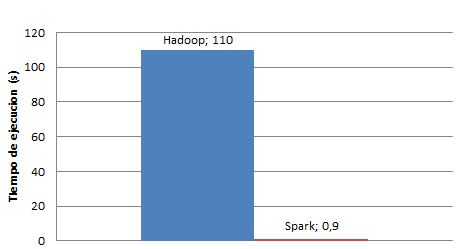
\includegraphics[width=0.7\textwidth]{./imagenes/comparacion_s_h}
	\caption{Tiempo de ejecución de Spark y Hadoop. \cite{Spark}} 
	
\end{figure}


Una de las principales diferencias entre Spark y Hadoop es que en Spark cada tarea puede tener un número indefinido de etapas de trabajo, mientras que en MapReduce solo teníamos dos etapas preestablecidas para cada tarea, Map y Reduce. Además, en Spark los resultados intermedios ofrecidos por las diferentes etapas pueden ser almacenados en memoria y no necesariamente en disco, como hacia MapReduce, aumentando así la velocidad de acceso a los datos.\\

Otro aspecto fundamental de Spark son los Resilient Distributed Dataset (RDD). Los RDDs son los objetos en los que Spark guarda la información leída de la fuente de datos. Una vez los datos han sido almacenados en objetos RDD, con Spark podemos realizar diferentes operaciones de procesamiento. Tenemos dos tipos de operaciones principales:\\

- \emph{Transformaciones}: Cuando hacemos una transformación a un RDD obtenemos un nuevo RDD modificado basado en el RDD original.\\

- \emph{Acciones}: Al hacer una acción sobre un RDD obtenemos un valor como resultado de la operación, que dependerá del tipo de operación que hayamos realizado.\\

Como hemos comentado anteriormente, los resultados intermedios de las transformaciones y de las acciones los podemos almacenar en memoria, de forma que si en una operación posterior necesitamos acceder a los resultados de las operaciones anteriores podamos acceder a ellos de forma rápida.\\

El modelo de procesamiento planteado por Spark se puede resumir del siguiente modo:\\

- En primer lugar leemos los datos de una fuente que puede ser un fichero de texto, por ejemplo, y los almacenamos en un objeto RDD.\\

- A partir del objeto RDD original creamos diferentes objetos RDD, de forma que tengamos la información almacenada de forma distribuida.\\
	
- Por último, podemos aplicar diferentes transformaciones  y acciones a los RDDs con el fin de obtener los resultados que buscamos, cuando tengamos el RDD final con los resultados lo podemos almacenar en disco.	

\begin{figure}[H]
	\centering
	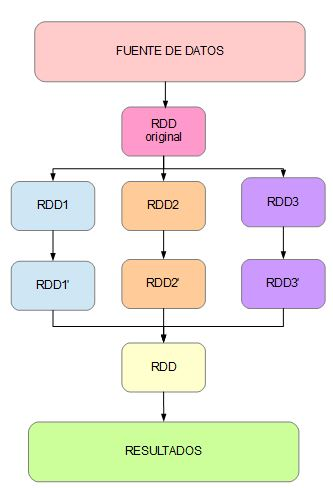
\includegraphics[width=0.7\textwidth]{./imagenes/programacion_spark}
	\caption{Modelo de procesamiento de Spark.} 
	
\end{figure}

Hay veces que necesitaremos tratar datos que se encuentren en diferentes RDD, para ello podemos distinguir dos tipos de transformaciones:\\

- \emph{Narrow transformation}: Se utiliza cuando los datos que necesitamos están en un mismo RDD, por lo que no necesitamos mezclar los datos de varios RDDs. Algunas de estas son las funciones filter() o sample().\\

- \emph{Wide tranformation}: Son las que se utilizan cuando se necesita consultar datos que están almacenados en diferentes RDDs y es necesario mezclarlos para agrupar los datos que queremos en un solo RDD. Algunas de estas transformaciones son groupByKey() o reduceByKey().\\

\begin{figure}[H]
	\centering
	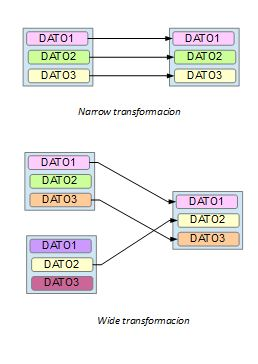
\includegraphics[width=0.7\textwidth]{./imagenes/transformaciones_spark}
	\caption{Diferentes transformaciones en Spark.} 
	
\end{figure}

